\documentclass[a4paper]{article}
\usepackage[pdftex]{graphicx}
\usepackage[utf8]{inputenc}
\usepackage{enumerate}
\usepackage{siunitx}
\sisetup{locale=DE}
\usepackage{icomma}
\usepackage{amssymb}
\usepackage{tikz}
\usepackage{href-ul}
\hypersetup{
	colorlinks=true,
	linkcolor=blue,
	urlcolor=blue}
\usepackage{geometry}
\geometry{a4paper, top=15mm, left=15mm, right=15mm, bottom=15mm,
	headsep=10mm, footskip=12mm}


\begin{document}
	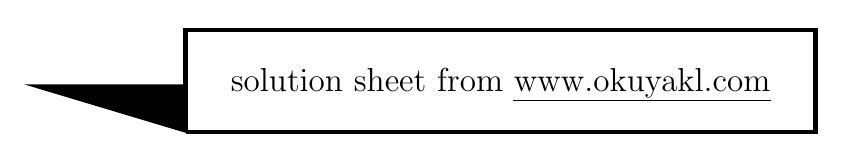
\begin{tikzpicture}(10,3)
		\draw[ultra thick](2,0) --(10,0) -- (10,1.3) --(2,1.3) -- (2,0);
		\draw[fill=black](2,0)-- (0,.6) -- (2,.6) -- (2,0);
		\node at (6,.6) {\large solution sheet from \href{http://www.okuyakl.com}{www.okuyakl.com}};
	\end{tikzpicture}
	\vspace{0.5 cm}
	
	
	\noindent
	\begin{minipage}{0.5\textwidth}
		\bf{Task 1. a)}\\
		\includegraphics[width=5 cm]{wike96.pdf}
	\end{minipage}
	\hfill
	\begin{minipage}{0.5\textwidth}
		\bf{Task 1. b)}\\
		\includegraphics[width=5 cm]{wili96.pdf}
	\end{minipage}
	
	\begin{tabular}{c|c|c|c|c|c|c|c|c|c}
		& $U$ in $\SI{}{\volt}$ & 0 & 0.30 & 0.60 & 0.90 & 1.20 & 1.50 & 1.80 & 2.10 \\
		\hline
		Iron wire & $I$ in $\SI{}{\ampere}$ & 0 & 0.48 & 0.93 & 1.38 & 1.70 & 1.98 & 2.19 & 2.31 \\
		& $R$ in $\SI{}{\ohm}$ & 0 & 0.63 & 0.65 & 0.65 & 0.70 & 0.76 & 0.82 & 0.91 \\
		\hline
		Constantan wire & $I$ in $\SI{}{\ampere}$ & 0 & 0.09 & 0.18 & 0.27 & 0.36 & 0.45 & 0.54 & 0.63 \\
		& $R$ in $\SI{}{\ohm}$ & 0 & 3.33 & 3.33 & 3.33 & 3.33 & 3.33 & 3.33 & 3.33 \\
		\hline
	\end{tabular}
	\vspace{10 pt}
	
	\noindent{\bf{Task 1. c)}}\\
	The conductor characteristic of iron is above that of constantan. It follows that the iron wire conducts better. If you compare the shape of the two curves, you will notice that the slope of the constantan line is the same everywhere, but the iron characteristic curve rises steeply and becomes flatter as the current intensity increases.
	However, as the current increases, both wires heat up. This means that constantan conducts equally well when warm and when cold, while iron conducts less well as the temperature increases. This is also proven by the calculated resistance values in the table.
	\vspace{0.5 cm}
	
	\noindent{\bf{Task 1. d)}}\\
	The electrical resistance of iron increases with temperature. The charge carriers are plentiful. Their movement, which is as straight as possible from one pole to the other, is disrupted as the atomic body's own motion increases.
	\vspace{0.5 cm}
	
	\noindent{\bf{Task 2.}}\\
	The additional resistor must conduct the larger current flow past the measuring device, i.e. be connected in parallel. The resistance value of the so-called shunt is calculated as follows:
	
	First, we calculate the voltage present at the ammeter at full scale:
	$$U_{max} = R \cdot I = \SI{3.0}{\milli\ampere} \cdot \SI{70}{\ohm} = \SI{0.21}{\volt}$$
	This voltage must now also be present at the ammeter when $$I_V=\SI{30}{\milli\ampere}-\SI{3,0}{\milli\ampere}=\SI{27}{\milli\ampere }$$
	flow past him through the shunt. Then the following applies to its resistance: $R_S$:
	$$R_S= {U_{max} \over I_V}={\SI{0.21}{\volt} \over \SI{0.027}{\ampere}}= \SI{7.8}{\ohm} $$
	\vspace{0.5 cm}
	
	\noindent{\bf{Task 3.}}\\
	You can count on an internal resistance in the same way as an ordinary resistance. The following voltage drops across the internal resistance of the starter battery:
	$$U_i= I \cdot R_i = \SI{120}{\ampere} \cdot \SI{0.030}{\ohm}= \SI{3.6}{\volt}$$
	This voltage must be subtracted from the source voltage to obtain the operating voltage $U_B$:
	$$ U_B = \SI{12}{\volt} - \SI{3.6}{\volt} = \SI{8.4}{\volt}$$
	This gives us the resistance $R_A$ of the starter:
	$$ R_A = {U_B \over I} = {\SI{8.4}{\volt} \over \SI{120}{\ampere}}=\SI{0.07}{\ohm}$$
	
	\vspace{0.5 cm}
	
	\noindent{\bf{Task 4. a)}}\\
	
	\noindent
	\begin{minipage}{0.6\textwidth}
		Minimum power:\\
		\includegraphics[width=10 cm]{wrei96.pdf}
	\end{minipage}
	\hfill
	\begin{minipage}{0.4\textwidth}
		Greatest achievement:\\
		\includegraphics[width=5 cm]{wpar96.pdf}
	\end{minipage}
	\vspace{0.5 cm}
	
	\noindent{\bf{Task 4. b)}}\\
	Smallest power = largest resistance = series connection:
	$$R_{rei}= \SI{50}{\ohm} + \SI{50}{\ohm} + \SI{50}{\ohm} = \SI{150}{\ohm} $$
	$$P_{rei}= U \cdot I = U \cdot {U\over R} = {U^2 \over R} = {(\SI{230}{\volt})^2 \over \SI{ 150}{\ohm}}= \SI{353}{\watt}$$
	Maximum power = smallest resistance = parallel connection:
	$$R_{par}= \left( {1\over \SI{50}{\ohm}} + {1\over\SI{50}{\ohm}} + {1\over \SI{50}{ \ohm}} \right)^{-1} = {50 \over 3}\SI{}{\ohm} = \SI{16,7}{\ohm} $$
	$$P_{par}={(\SI{230}{\volt})^2 \over \SI{16.7}{\ohm}}= \SI{3170}{\watt}$$
	
	\begin{center}
		\includegraphics[width=7 cm]{../../viecher/eendcomic.pdf}
		
		Here you can go back to the \href{https://www.okuyakl.de/phys/p10elL096/ae096.pdf}{task sheet}
	\end{center}
	
\end{document}